% !TeX encoding = UTF-8
% !TeX spellcheck = en_US

\definecolor{couleurback}{HTML}{CCFFCC}

\section{CirJSON Values}

A CirJSON value can be an \textit{object}, \textit{array}, \textit{number}, \textit{string}, \texttt{true}, \texttt{false}, or \texttt{null}, \textit{ID}.

\begin{figure}[!htbp]
	\centering
	\tikzset{
		val/.style={draw, fill=couleurback, thick, text width=6em, align=flush center,line width=2pt},
		lit/.style={val, rounded corners=8pt},
	}
	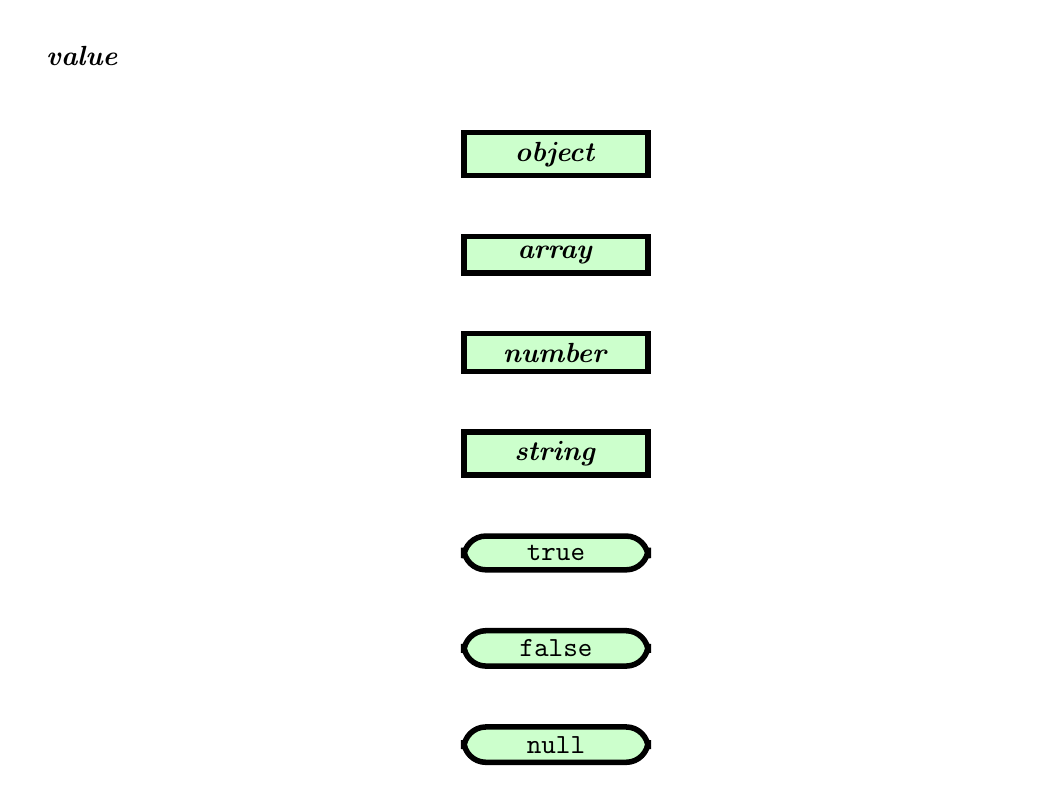
\begin{tikzpicture}[line width=2pt]
		\matrix[row sep=2em, column sep=12em] {
			\node{\textbf{\textit{value}}}; & ~ & ~ \\
			\node(start){~}; & \node[val](obj){\textbf{\textit{object}}}; & \node(end){~}; \\
			~ & \node[val](arr){\textbf{\textit{array}}}; & ~ \\
			~ & \node[val](num){\textbf{\textit{number}}}; & ~ \\
			~ & \node[val](str){\textbf{\textit{string}}}; & ~ \\
			~ & \node[lit](tr){\textbf{\texttt{true}}}; & ~ \\
			~ & \node[lit](fl){\textbf{\texttt{false}}}; & ~ \\
			~ & \node[lit](nl){\textbf{\texttt{null}}}; & ~ \\
		};
		
		\multiLinksRight{start}{obj,arr,num,str,tr,fl,nl}
		\multiLinksLeft{obj,arr,num,str,tr,fl,nl}{end}
	\end{tikzpicture}
	\caption{CirJSON Values}
	\label{f:vals}
\end{figure}

\begin{tikzpicture}[->,shorten >=1pt,auto,node distance=3cm,semithick]
	\tikzstyle{every state}=[draw=black,text=black]
	
	\node[initial by arrow,state,initial text=] (1) {1};
	\node[state] (3) [right of=1] {3};
	\node[accepting,state] (4) [below of=1] {4};
	\node[state] (2) [below of=4] {2};
	\node[state] (5) [right of=2] {5};
	\node[state] (6) [right of=4] {6};
	\node[state] (7) [below of=2] {7};
	
	\path
	(1) edge node {$a$} (4)
	(1) edge node {$b$} (3)
	(2) edge node {$a$} (7)
	(2) edge node {$b$} (5)
	(3) edge node {$a$} (4)
	(3) edge node {$b$} (6)
	(4) edge node {$a$} (2)
	(4) edge node {$b$} (5)
	(5) edge node {$a$} (7)
	(5) edge node {$b$} (6)
	(6) edge node {$a$} (4)
	(6) edge [loop right] node {$b$} (6)
	(7) edge [loop left] node {$a,b$} (7)
	;
	
\end{tikzpicture}
